%    Documentation for PRU ADC Project
%    Copyright (C) 2016  Gregory Raven
%
%    This program is free software: you can redistribute it and/or modify
%    it under the terms of the GNU General Public License as published by
%    the Free Software Foundation, either version 3 of the License, or
%    (at your option) any later version.
%
%    This program is distributed in the hope that it will be useful,
%    but WITHOUT ANY WARRANTY; without even the implied warranty of
%    MERCHANTABILITY or FITNESS FOR A PARTICULAR PURPOSE.  See the
%    GNU General Public License for more details.
%
%    You should have received a copy of the GNU General Public License
%    along with this program.  If not, see <http://www.gnu.org/licenses/>.

\chapter{User Space Program: Fork and Named Pipe}

	\begin{figure}[h]
		\centering
		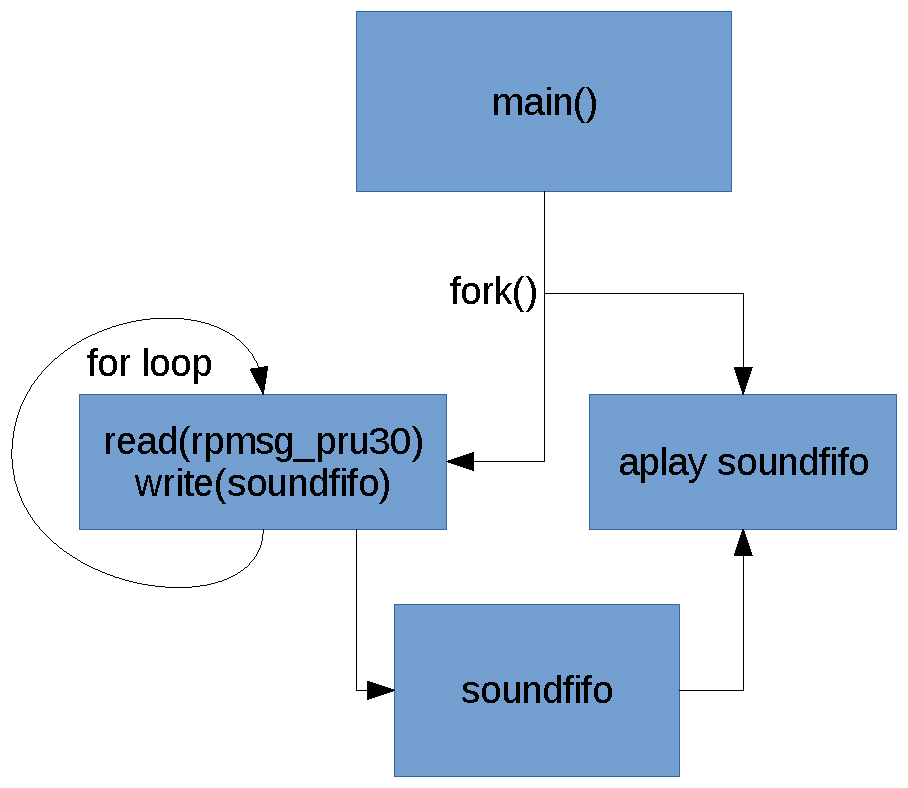
\includegraphics[width=0.8\textwidth]{diagrams/fork-crop}
		\centering\bfseries
		\caption{Data Flow in User Space Program}
	\end{figure}
	
	
	The user-space program is responsible for reading the data from PRU0 and then writing that data to ALSA.
	This requires the program to create two separate processes and some facility to allow data to flow from one process to the other.
	
	The system call to fork() combined with a ``named pipe'' implements these features in a user-space C program.
	
	Note that the user-space program does not create the named pipe.  A command in the Makefile creates the named pipe in the same directory as the user-space executable.  The named pipe appears in the file system and can be seen with the usual ls command.